

\documentclass{article}
\usepackage[utf8]{inputenc}
\usepackage[utf8]{inputenc}
\usepackage[T1]{fontenc}
\usepackage[english]{babel}
\usepackage{fullpage}
\usepackage{color}
\usepackage[table]{xcolor}
\usepackage{listings}
 
\definecolor{darkWhite}{rgb}{0.94,0.94,0.94}
 
\lstset{
  aboveskip=3mm,
  belowskip=-2mm,
  backgroundcolor=\color{darkWhite},
  basicstyle=\footnotesize,
  breakatwhitespace=false,
  breaklines=true,
  captionpos=b,
  commentstyle=\color{red},
  deletekeywords={...},
  escapeinside={\%*}{*)},
  extendedchars=true,
  framexleftmargin=16pt,
  framextopmargin=3pt,
  framexbottommargin=6pt,
  frame=tb,
  keepspaces=true,
  keywordstyle=\color{blue},
  language=C,
  literate=
  {²}{{\textsuperscript{2}}}1
  {⁴}{{\textsuperscript{4}}}1
  {⁶}{{\textsuperscript{6}}}1
  {⁸}{{\textsuperscript{8}}}1
  {€}{{\euro{}}}1
  {é}{{\'e}}1
  {è}{{\`{e}}}1
  {ê}{{\^{e}}}1
  {ë}{{\¨{e}}}1
  {É}{{\'{E}}}1
  {Ê}{{\^{E}}}1
  {û}{{\^{u}}}1
  {ù}{{\`{u}}}1
  {â}{{\^{a}}}1
  {à}{{\`{a}}}1
  {á}{{\'{a}}}1
  {ã}{{\~{a}}}1
  {Á}{{\'{A}}}1
  {Â}{{\^{A}}}1
  {Ã}{{\~{A}}}1
  {ç}{{\c{c}}}1
  {Ç}{{\c{C}}}1
  {õ}{{\~{o}}}1
  {ó}{{\'{o}}}1
  {ô}{{\^{o}}}1
  {Õ}{{\~{O}}}1
  {Ó}{{\'{O}}}1
  {Ô}{{\^{O}}}1
  {î}{{\^{i}}}1
  {Î}{{\^{I}}}1
  {í}{{\'{i}}}1
  {Í}{{\~{Í}}}1,
  morekeywords={*,...},
  numbers=left,
  numbersep=10pt,
  numberstyle=\tiny\color{black},
  rulecolor=\color{black},
  showspaces=false,
  showstringspaces=false,
  showtabs=false,
  stepnumber=1,
  stringstyle=\color{gray},
  tabsize=4,
  title=\lstname,
}
\usepackage{graphicx}
\title{HAI804I – Codage et compression multimédia
}
\author{Fabien Caballero}

\begin{document}

\maketitle
    \tableofcontents

\newpage

\begin{figure}[h]
%\centerline{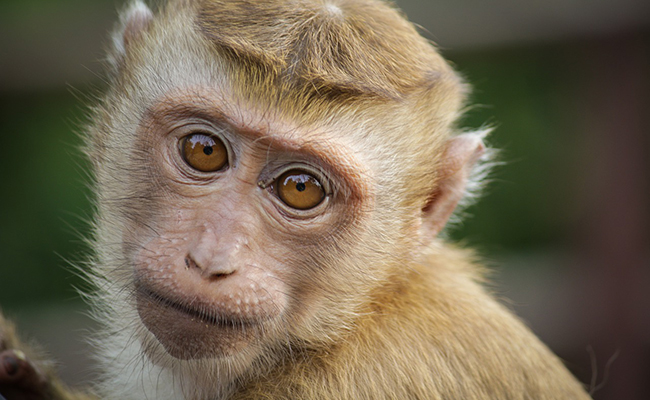
\includegraphics[scale=0.3]{./rendus/singe.jpg}}
\caption{Image d'origine utilisée tout le long du TP}
\end{figure}

\addcontentsline{toc}{section}{Introduction}
\section*{Introduction}
Le but de ce TP est d’appliquer une transformée en ondelettes sur une image afin de la
compresser.
\\\\
\section{Compression d'une image pgm avec une transformée en ondelettes}
\subsection{4 sous bande, une itération}
\begin{figure}[h!]
\centerline{ 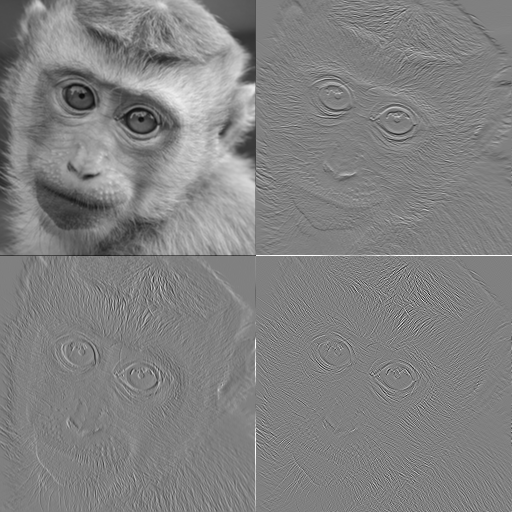
\includegraphics[scale=0.5]{./rendus/4sousBandes1iterPGM.png} }
\caption{4 sous bandes de Haar (BF Haut gauche, HF Haut droite, HBF Bas gauche, BHF Bas droite)} 
\end{figure}

\newpage
\subsection{Reconstruction à partir des 4 sous bandes, une itération}
\begin{figure}[h!]
\centerline{ 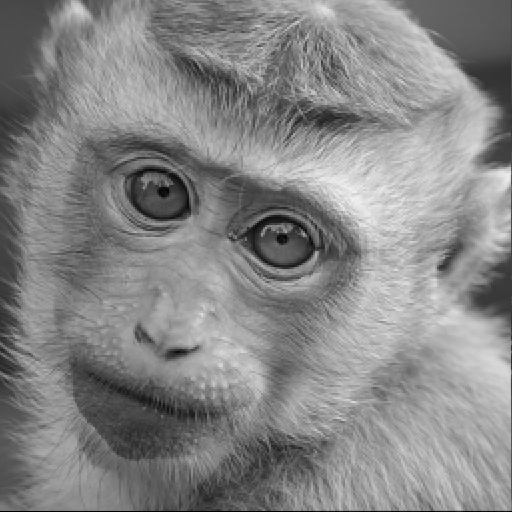
\includegraphics[scale=0.5]{./rendus/Reconstruite1.png} }
\caption{Image reconstruite (512x512) avec les 4 sous bandes d'une itération} 
On obtient un PSNR de 28.6401
\end{figure}



\newpage
\subsection{Quantification avec Q avec chaque coefficient variant}
\begin{figure}[h!]
\centerline{ 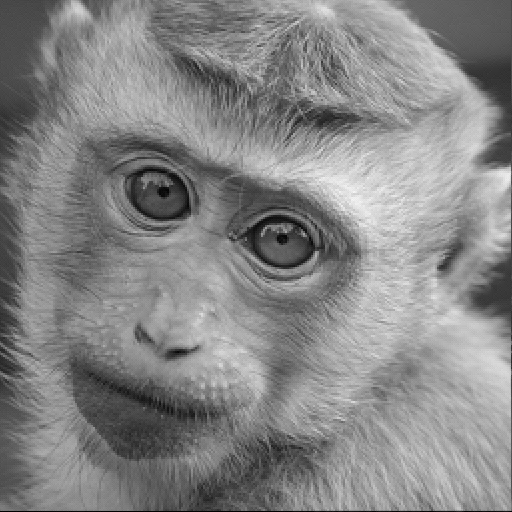
\includegraphics[scale=0.5]{./rendus/ReconstruiteQuantificationCoeff1_4_4_16.png} }
\caption{Quantification des sous bandes avec QBF=1, QMFh=4, QMFv=4, QHF=16} 
On obtient un PSNR de 28.229
\end{figure}


\begin{figure}[h!]
\centerline{ 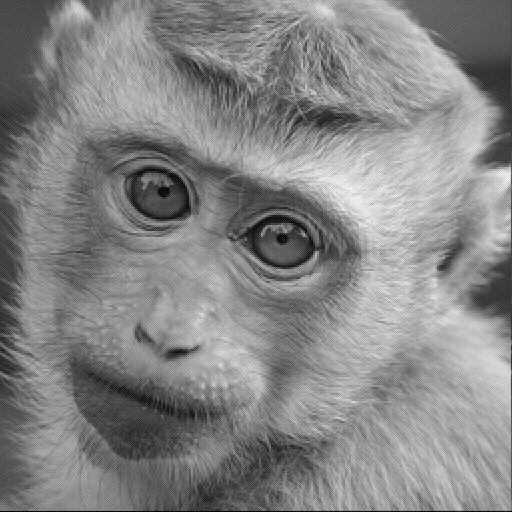
\includegraphics[scale=0.5]{./rendus/ReconstruiteQuantificationCoeff2_8_8_64.png} }
\caption{Quantification des sous bandes avec QBF=2, QMFh=8, QMFv=8, QHF=64} 
On obtient un PSNR de 25.0547
\end{figure}


\begin{figure}[h!]
\centerline{ 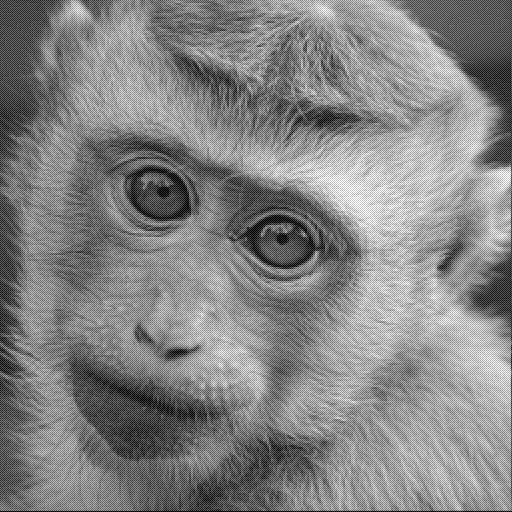
\includegraphics[scale=0.5]{./rendus/ReconstruiteQuantificationCoeff4_16_16_256.png} }
\caption{Quantification des sous bandes avec QBF=4, QMFh=16, QMFv=16, QHF=256} 
On obtient un PSNR de 17.5512
\end{figure}

\newpage
\subsection{Transformée en ondelettes avec un nombre décomposition variant}

\begin{figure}[h!]
\centerline{ 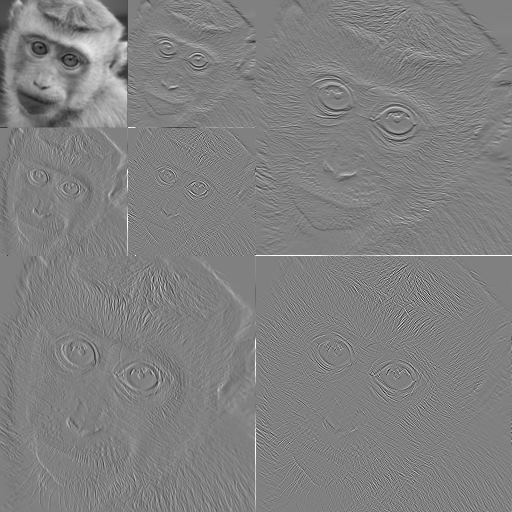
\includegraphics[scale=0.5]{./rendus/4sousBandes2iterPGM.png} 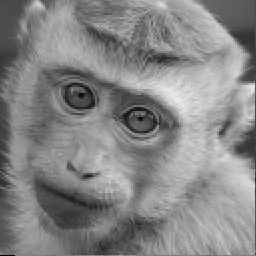
\includegraphics[scale=1]{./rendus/Reconstruite2.png} }
\caption{Pour 2 itérations sous bandes et image reconstruite (256x256) à droite} 
On obtient un PSNR de 29.4865
\end{figure}



\begin{figure}[h!]
\centerline{ 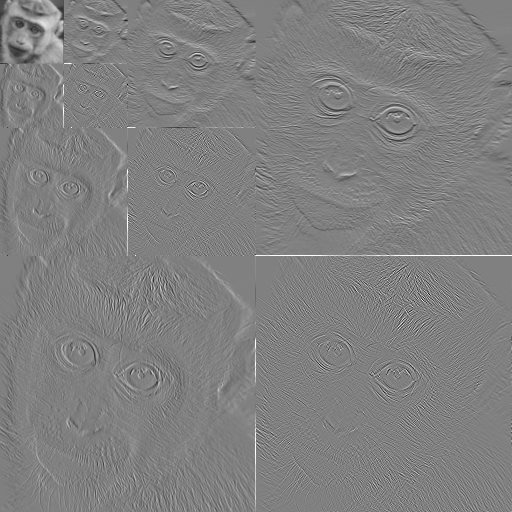
\includegraphics[scale=0.5]{./rendus/4sousBandes3iterPGM.png} 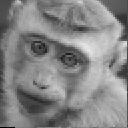
\includegraphics[scale=2]{./rendus/Reconstruite3.png} }
\caption{Pour 3 itérations  sous bandes et image reconstruite (128x128) à droite} 
On obtient un PSNR de 28.9968
\end{figure}



\begin{figure}[h!]
\centerline{ 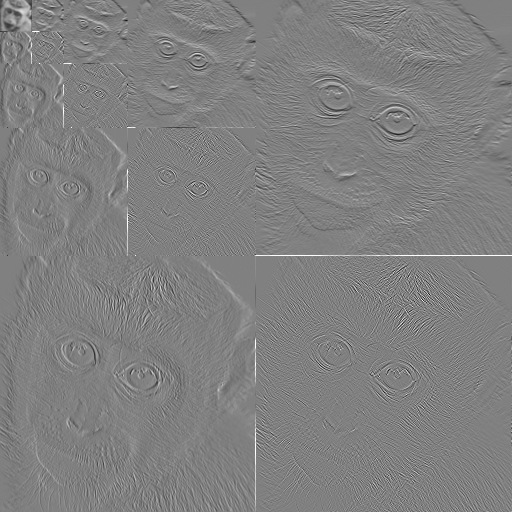
\includegraphics[scale=0.5]{./rendus/4sousBandes4iterPGM.png} 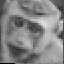
\includegraphics[scale=4]{./rendus/Reconstruite4.png} }
\caption{Pour 4 itérations  sous bandes et image reconstruite (64x64) à droite} 
On obtient un PSNR de 26.1428
\end{figure}



\begin{figure}[h!]
\centerline{ 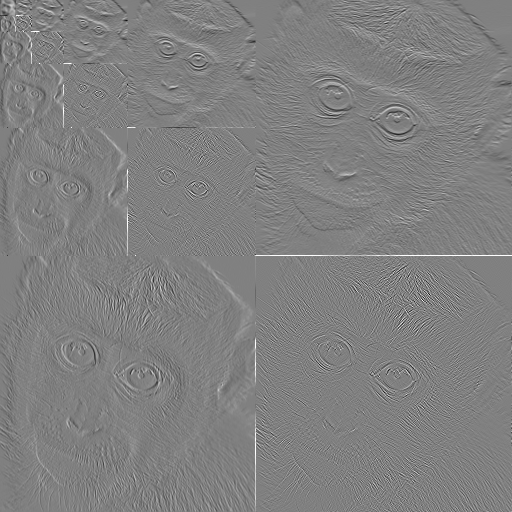
\includegraphics[scale=0.5]{./rendus/4sousBandes5iterPGM.png} 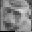
\includegraphics[scale=8]{./rendus/Reconstruite5.png} }
\caption{Pour 5 itérations  sous bandes et image reconstruite (32x32) à droite} 
On obtient un PSNR de 23.1367
\end{figure}



\begin{figure}[h!]
\centerline{ 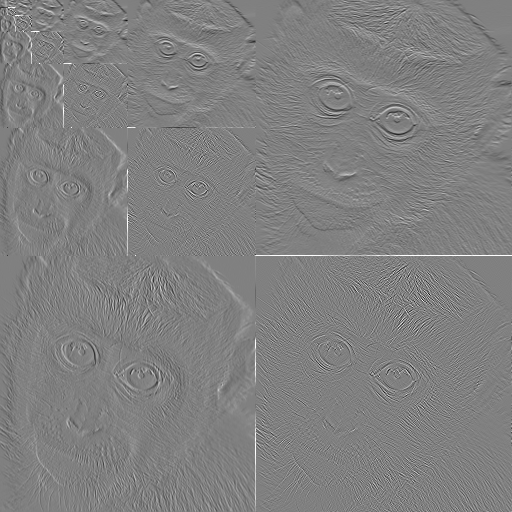
\includegraphics[scale=0.5]{./rendus/4sousBandes6iterPGM.png} 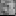
\includegraphics[scale=16]{./rendus/Reconstruite6.png} }
\caption{Pour 6 itérations  sous bandes et image reconstruite (16x16) à droite} 
On obtient un PSNR de 19.1217
\end{figure}


\newpage
\subsection{Codage sans perte pour chacune des sous bandes}
On peut utiliser un codage d'Huffman, et/ou un codage par plage.

\subsection{Courbes débit/distorsion}
En utilisant Huffman on obtient la courbe débit distorsion suivante
\begin{figure}[h!]
\centerline{ 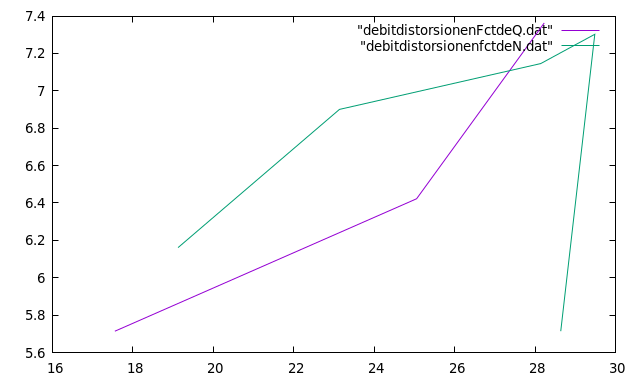
\includegraphics[scale=0.5]{./rendus/debit.png}}
\caption{Courbe de débit}
\end{figure}
Le résultat ne me semble pas correct.
Je ne pense pas avoir compris comment générer la courbe.

\end{document}